\section{Hardware}
\label{Sec:5-hardware}
\subsection{Raspberry - Sistema Operacional}

Raspberry Pi é um computador, como tal é possível usá-lo sobre um sistema operacional. O sistema operacional usado é o Raspian, baseado no Debian customizado para rodar no raspberry pi. Apesar de, teóricamente, não ser necessário o raspberry usar um sistema operacional, facilita muito o desenvolvimento tal equipamento conter uma interface amigável para para seu uso.

\subsection{Raspberry - Adaptador Wifi}

Após o sistema Raspian ser instalado no cartão de memória, foi necessário configurar o adaptador Wifi. O modelo usado é o TP-Link TL-WN723N.

\subsubsection{Procedimentos}
\begin{lstlisting}
wget https://dl.dropboxusercontent.com/u/80256631/8188eu-3.18.11-v7-781.tar.gz
tar xzf 8188eu-3.18.11-v7-781.tar.gz
./install.sh
\end{lstlisting}

\begin{figure}[H]
\centering
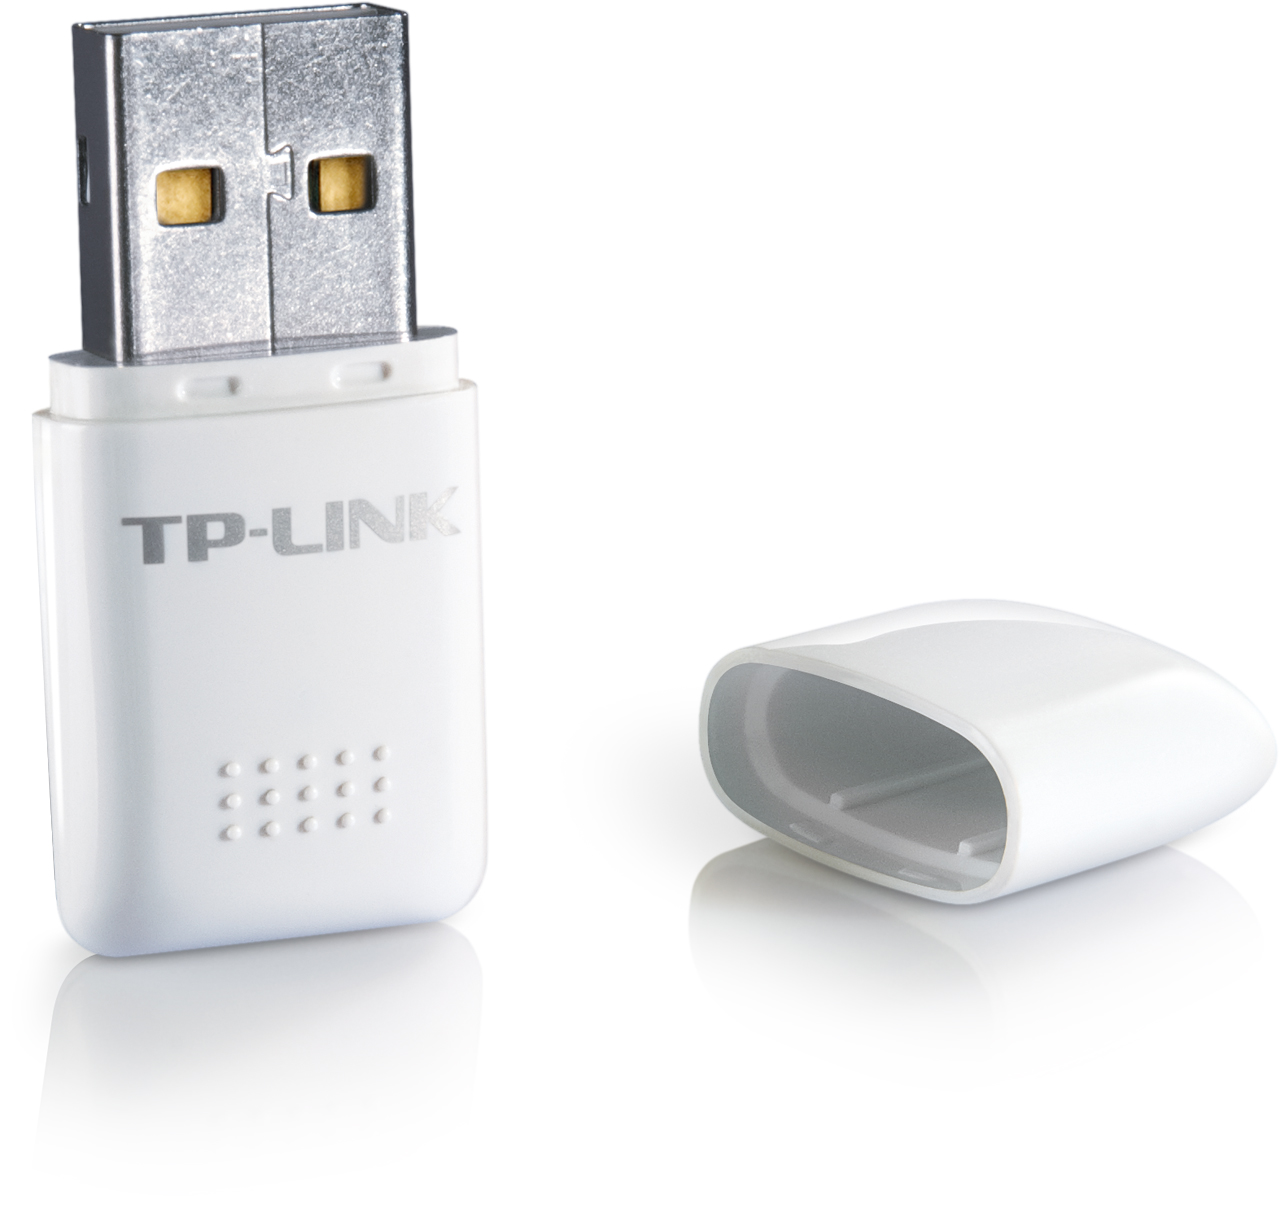
\includegraphics[width=5cm,height=5cm,keepaspectratio]{figuras/wifi-adapter.jpg}
\caption{\label{fig:wifi-adapter} Adaptador wifi usado no raspberry}
\end{figure}

\subsection{Testes iniciais}

Para testar a comunicação entre o Raspberry e o Arduino, executamos dois programas. O programa  foi utilizado no Arduino para transmitir o valor "123123" por um datagrama a ser enviado pela rede do XBee. Já o programa  foi utilizado no Raspberry para receber o datagrama ZigBee e imprimir no console.

\lstinputlisting[language=C, caption=teste1-arduino.c, label={lst:teste1-arduino}]{Anexos/teste1-arduino.c}

\lstinputlisting[language=python, caption=teste1-raspberry.py, label={lst:teste1-raspberry}]{Anexos/teste1-raspberry.py}

\begin{figure}[H]
\centering
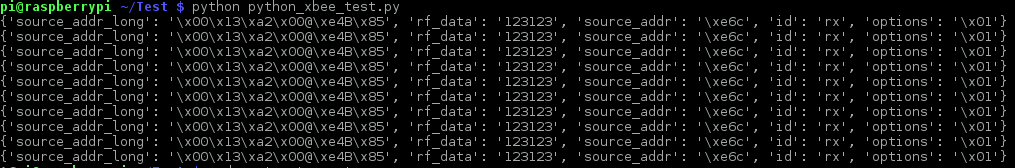
\includegraphics[width=1\textwidth]{figuras/raspberry_arduino_1.png}
\caption{\label{fig:raspberry_arduino_1} Teste de comunicação Raspberry e Arduino}
\end{figure}